% BEGIN (PARALLELISATION)
% ===========================================================================
\subsection{Overview}

Within a FLAME simulation, every agent only interacts with its environment via the reading and writing of messages to a collection of Message Boards. This makes the Message Board component an ideal candidate for enabling parallelism. 

Using distributed Message Boards, agents can be farmed out across multiple processing nodes and simulated in parallel while coherency of the simulation is maintained through a unified view of the distributed Boards.

\begin{figure}[ht]
 \centering
  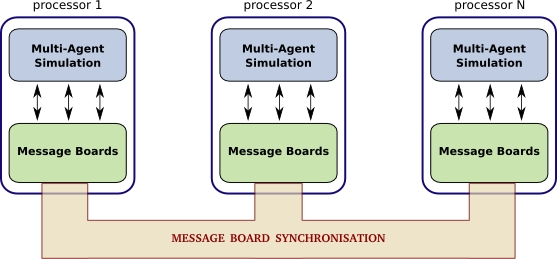
\includegraphics[scale=0.60]{mboard_flame.jpg}
 \caption{Parallelisation of FLAME using distributed Message Boards}
 \label{fig:mb_flame}
\end{figure}

\subsection{The Message Board library}
In the recent code release, the Message Board was decoupled from the FLAME framework and implemented as a separate library. This provided the flexibility to experiment with different parallelisation strategies while minimising the impact on current users of the FLAME framework.

\begin{figure}[ht]
 \centering
  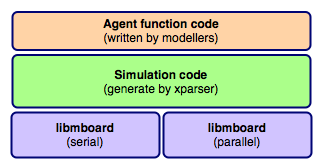
\includegraphics[scale=0.60]{mboard_overview.png}
 \caption{Users can create either serial or parallel executables by linking their object files to the appropriate \textit{libmboard} library}
 \label{fig:mb_overview}
\end{figure}

The Message Board Library (\textit{libmboard}) can be built as a set of static libraries which are linked to users' simulation object files to create serial and parallel executables. This setup enables users to maintain a common source base for both serial and parallel simulations, thus simplifying code management and testing. It also provides \textit{libmboard} developers the facility to quickly switch between different library implementations without having to constantly recompile the test program.

All functionality provided by the Message Board Library is accessible via the \textit{libmboard} Application Program Interface (API) which defines a set of routines and opaque datatypes. Through the API, the full functionality of the library is made available without exposing the internal implementation. With this separation between interface and implementation, the complete communication strategy and data representation system can be replaced without the users being affected. This level of flexibility is crucial in the EURACE project as \textit{libmboard} is being developed in tandem with modelling activities that require a working implementation.

Within the FLAME framework, the \textit{libmboard} API is used only by the framework-generated routines and not directly by the modellers. Modellers are provided with model-specific routines that hide the complexity of managing boards and packaging data into suitable datatypes. Figure~\ref{fig:mb_api_flame} shows an example of this whereby an agent's message add request gets translated into a \textit{libmboard} API call.

\begin{figure}[ht]
 \centering
  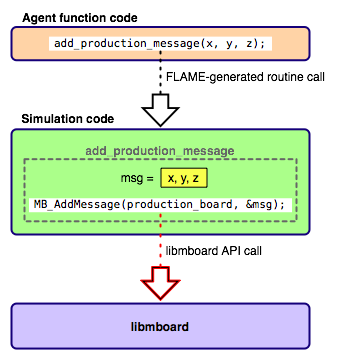
\includegraphics[scale=0.60]{mboard_codetranslate.png}
 \caption{Modellers use FLAME-generated routines which gets translated to the appropriate \textit{libmboard} API call}
 \label{fig:mb_api_flame}
\end{figure}


\textit{libmboard} uses the Message Passing Interface (MPI) to communicate between processors, and POSIX threads (pthreads) to manage a separate thread for handling data management and inter-process communication. Further details are available in Section~\ref{sec:mb_sync} and Section~\ref{sec:commthread}.

% ===========================================================================
\subsection{The \textit{libmboard} API}
\label{sec:mb_api}

The  \textit{libmboard} API is intended for use within the FLAME generated simulation code. It provides the functionality for creating, managing and accessing Message Boards. Implementation details such as internal data representations, memory management and communication strategies are transparent to API users and therefore can be replaced or improved without affecting FLAME developers and end-users.

In the following sections we discuss the use of Boards, Iterators and Synchronisation. For further details, refer to the \textit{libmboard} Reference Manual\cite{MessageBoardAPI} which includes the full API specification and usage example.
% ---------------------------------------------------------------------------
%\subsubsection{Library environment}

%\begin{itemize}
%\item Init and finalise
%\item MPI env
%\item fork/join comm thread thread
%\end{itemize} 

% ---------------------------------------------------------------------------
\subsubsection{Boards}

Message Boards are essentially distributed data structures that can be read from and written to by agents on all processing nodes. Up to 4096 different Message Boards can be created, whereby each Board is created to store message objects of a specified size.

Message Boards are created using the \texttt{MB\_Create()} routine. This routine will return a Board Handle (of type \texttt{MBt\_Board}) which can be used to reference the Board when performing further operations.

Once a Board is created, messages can be added to it using the \texttt{MB\_AddMessage()} routine. During an add, the message data is duplicated and stored in the Board, allowing the calling code to reuse or deallocate the original message data. The cloning of data greatly simplifies the usage of the API and protects the internal data representation from accidental corruption. 

Messages added to the Board are immediately available to all agents within the local processing node, or, after a sync (see Section~\ref{sec:mb_sync}), across all processing nodes.

The API provides further routines from emptying (\texttt{MB\_Clear()}) and deleting  (\texttt{MB\_Delete()}) Boards.

% ---------------------------------------------------------------------------
\subsubsection{Iterators}
\label{sec:mb_iterators}

Iterators are opaque objects used for traversing Message Board content. They provide \textit{libmboard} users access to messages while isolating them from the internal data representation of Boards. It also aids in enforcing the rule that Boards should be not modified in any way by a read access. With this rules in place, multiple Iterators can be created to traverse the Board independently using different access patterns.

\begin{figure}[ht]
 \centering
  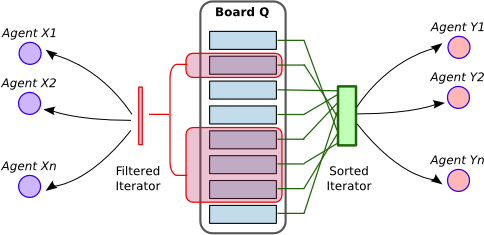
\includegraphics[scale=0.8]{iterator.png}
 \caption{Using specialised Iterators to achieve different access patterns}
 \label{fig:mb_iterators}
\end{figure}

Iterators are created against a Board using the \texttt{MB\_Iterator\_Create()} routine. Upon creation, the Iterator generates a list of the available messages within the Board and places a cursor at the first entry. When an Iterator is created, it essentially creates a snapshot of the content of a local Board. Any data added to the Board after the creation of the Iterator will not be available, while emptying or deleting the Board will invalidate the Iterator.

Data traversal is performed by repeated calls to \texttt{MB\_Iterator\_GetMessage()}. This routine returns a copy of a single message data, then moves the cursor to the next item. Once the cursor moves beyond the last item, further calls to \texttt{MB\_Iterator\_GetMessage()} will return a \texttt{NULL} pointer indicating that iteration has ended. \texttt{MB\_Iterator\_Rewind()} can be used to move the cursor back to the first item to allow for a reuse of the Iterator.

The \textit{libmboard} API also provides several routines for creating specialised Iterators which allow users to traverse subsets of the Board content in a customised order. These routines accept user-defined sort and/or compare functions that are used to control the selection of messages and their order in the Iterator. These specialised Iterators are traversed just like a standard Iterator, using \texttt{MB\_Iterator\_GetMessage()}.

Other Iterator routines include \texttt{MB\_Iterator\_Randomise()} for randomising Iterator entries, and \texttt{MB\_Iterator\_Delete()} for deleting Iterators.

%\begin{itemize}
%\item isolate users from internal data representation
%\item normal/filtered/sorted
%\item returning cloned mem vs ptr.
%\item randomisation
%\item rewind
%\end{itemize} 

% ---------------------------------------------------------------------------
\subsubsection{Synchronisation}
\label{sec:mb_sync}

Synchronisation of Boards involves the propagation of message data such that agents farmed out across the different processing nodes have a unified view of the collective content through their local Boards. This is vital to ensure that the simulation is coherent even though instances of the Board are distributed across different processing nodes.

Synchronisation of Boards is performed in two stages -- the initial Board synchronisation request, and the actual completion of synchronisation.

The initial Board synchronisation request is performed using \texttt{MB\_SyncStart()}. This routine locks the Board and adds it to the \textit{Synchronisation Request Queue} (discussed in Section~\ref{sec:syncqueue}). The calling code is then immediately given back control and is free to proceed with other tasks that do not require access to the Board in question. 

When read access to the Board is required, the synchronisation process must first be completed using \texttt{MB\_SyncComplete()}. This routine is blocking, and will wait for the Board to be unlocked before returning control to the calling code. Alternatively, there is also the \texttt{MB\_SyncTest()} routine which is non-blocking and returns immediately with the completion status of the synchronisation. The calling code can immediately access the Board if the returned status is \texttt{MB\_TRUE}, or, if the returned status is \texttt{MB\_FALSE}, proceed with other tasks and repeat the test at a later stage.

The sequence diagram in  Figure~\ref{fig:syncboard} depicts how a board synchronisation request may take place. The process of actually synchronising and unlocking the board is performed concurrently in the background by the \textit{Communication Thread}. This is discussed further in Section~\ref{sec:commthread}.

\begin{figure}[ht]
 \centering
  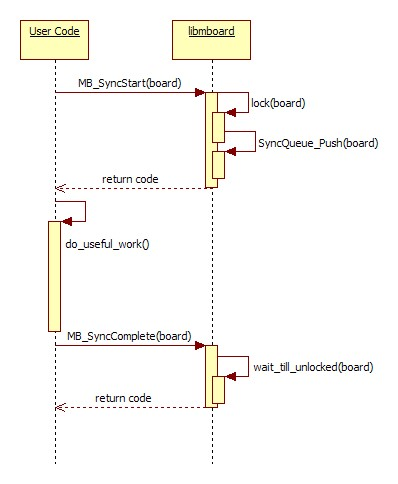
\includegraphics[scale=0.60]{syncboard.jpg}
 \caption{Other work can be scheduled during board synchronisation to hide the overheads of communication}
 \label{fig:syncboard}
\end{figure}

To make the most of the concurrent nature of \textit{libmboard}, calls to \texttt{MB\_SyncStart()} should be placed as early as possible within the code (immediately after the final message has been written) such that more work can be scheduled before \texttt{MB\_SyncComplete()} is called. This will maximise the amount of overlap between useful computation and the synchronisation overheads.

% ---------------------------------------------------------------------------
\subsubsection{Sync optimisation based on Message Tagging}
\label{sec:mb_tagging}

In its simplest form, a Board synchronisation may be implemented as a full replication of all messages within each local Board. This method is rather straightforward to implement, and would indeed serve its purpose of providing every agent access to the collective Board content. Unfortunately, it is also extremely expensive in terms of communication and memory requirements, and would therefore defeat the purpose of running in parallel (considering the key reasons behind parallelisation are to reduce elapsed time and per-node memory usage).

\textit{libmboard} overcomes this problem by tagging each message with the IDs of processing nodes that require read access to it (see Figure~\ref{fig:taggedboard}). With the tagging in place, full data replication is avoided by only propagating the relevant messages to each processing node.

\begin{figure}[ht]
 \centering
  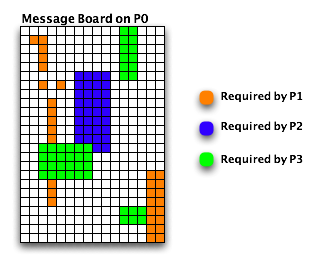
\includegraphics[scale=0.70]{taggedboard.png}
 \caption{Full data replication is avoided by only propagating tagged messages to the relevant nodes}
 \label{fig:taggedboard}
\end{figure}

In order to tag messages, each processing node would need to indicate the selection of messages that it requires. This facility is provided by the  \texttt{MB\_Function\_Assign()} routine which assigns used-defined filter functions and their associated parameters to each Board . At the start of each synchronisation, the parameters are gathered from all remote nodes and message tagging is performed.

Within the FLAME framework, the filter functions are generated automatically based on the \texttt{<filter>} tag that modellers assign to the input of each agent function, while the function parameters are computed at run-time based on an analysis of agent memory. 

Obviously, if the \texttt{<filter>} tags are not used, filter functions will not be assigned to Boards and the synchronisation process would fall back to a full data replication.

% ===========================================================================
\subsection{The Communication Thread}
\label{sec:commthread}

During the initialisation of the Message Board environment, \textit{libmboard} starts up a separate thread (the \textit{Communication Thread}) to handle the synchronisation of distributed boards. 

Apart from potentially making better use of multi-core processors, delegating communication and memory intensive operations to a separate thread allows us to minimise the effective overheads by performing them concurrently with the main simulation and thus overlapping the Board synchronisation time with that of useful computation.

\begin{figure}[ht]
 \centering
  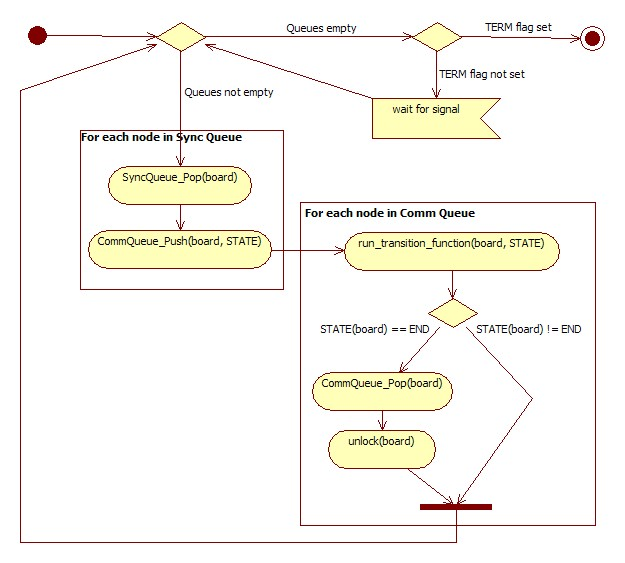
\includegraphics[scale=0.60]{commloop.jpg}
 \caption{Activity diagram for Communication Thread}
 \label{fig:commloop}
\end{figure}

Once the \textit{Communication Thread} is started, it goes into a continuous loop of processing two control queues -- the Synchronisation Request Queue (\textit{Sync Queue}), and the Pending Communication Queue (\textit{Comm Queue}). 

The loop is interrupted whenever both queues are empty, whereby the thread sleeps till it receives a signal from the parent thread, or quits when the termination flag is set. This is depicted by the Activity Diagram in Figure~\ref{fig:commloop}.

% ---------------------------------------------------------------------------
\subsubsection{The Sync Queue}
\label{sec:syncqueue}

The \textit{Sync Queue} is the interface between the \textit{Communication Thread} and parent thread, and acts as a staging point for Boards synchronisation requests. Boards that need to be synchronised are locked by the main thread and pushed into the \textit{Sync Queue} for further action by the \textit{Communication Thread}. Access to the queue is protected by the mutex lock mechanism provided by the \textit{pthreads} API.

When the \textit{Sync Queue} is processed, all Boards within the queue are placed in an appropriate state\footnote{depending on whether filter functions and parameters have been assigned to the Board} and moved into the \textit{Comm Queue}. The individual Board will remain locked until it has passed through the \textit{Comm Queue}.

% ---------------------------------------------------------------------------
\subsubsection{The Comm Queue}

The \textit{Comm Queue} manages the list of Boards that are in the midst of synchronisation. Each Board within the \textit{Comm Queue} is assigned a state based on the synchronisation stage it is in. Whenever the \textit{Comm Queue} is processed, the \textit{Communication Thread} iterates through the list of Boards and executes the transition function associated with the state of each Board. 

Boards that reach their \texttt{END} state are removed from the \textit{Comm Queue} and unlocked to indicated that synchronisation is complete. The unlocking of the board would be picked up by the parent thread when the appropriate libmboard API routines are called (refer back to Figure~\ref{fig:syncboard} for further clarification).

% ---------------------------------------------------------------------------
\subsubsection{Stages of synchronisation}

The synchronisation process of a Board is split into stages such that inter-process communication (non-blocking MPI sends and receives) spans across at least two state transition functions -- one to initialise the non-blocking send/receive operation, and the others to test and complete the communication.

For example, when a Board is in the \texttt{PRE\_PROPAGATION} state (see Board synchronisation state diagram in  Figure~\ref{fig:commstate}), the \texttt{InitPropagation()} transition function will prepare the necessary buffers, issue a series of non-blocking MPI sends and receives, and transition the Board to the \texttt{PROPAGATION} state without waiting for the communication to complete. During the next iteration, the \textit{Communication Thread} would come back to the same board and either transition it to the next state if all communication has completed, or maintain the state if there are still pending communications. 

\begin{figure}[ht]
 \centering
  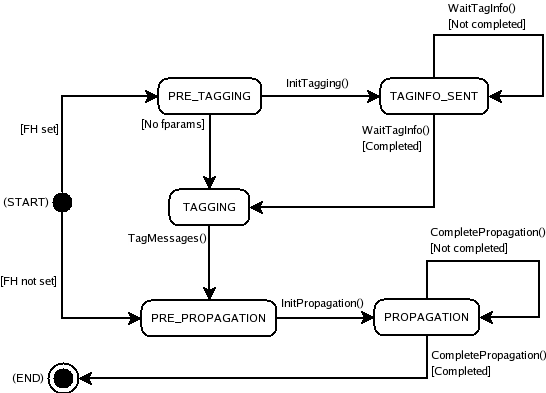
\includegraphics[scale=0.50]{CommNode.png}
 \caption{State diagram for processing Comm Queue nodes}
 \label{fig:commstate}
\end{figure}

By ensuring that transition functions never involve idle waits for events or specific conditions, the \textit{Communication Thread} can continuously cycle through all pending synchronisations and perform the transition of each Board as they are ready.

% ===========================================================================
\subsection{Issues}

\subsubsection{Use of \textit{pthreads}}

During the design stage of \textit{libmboard}, several complications were identified when considering the use of  \textit{pthreads} for implementing the \textit{Communication Thread}. It was eventually decided that the possibilities brought about by using a threaded model  outweigh the potential drawbacks. Some of the issues that were recognise are:
\begin{itemize}
\item Portability -- some platforms do not natively support \textit{pthreads}. For example, \textit{pthreads} are not supported on the IBM Bluegene/L system. They are also not available natively on Microsoft Windows Operating Systems. However, \textit{pthreads} support has been introduced in the latest generation of Bluegene (Bluegene/P), and on Windows, \textit{pthreads} can be used through Cygwin or by using third-party libraries.
\item Thread-safety -- Not all MPI Libraries currently available are thread-safe. This made the development of \textit{libmboard} much harder as this introduces an additional limitation that the parent thread (which includes the calling code and the API routines themselves) must not issue MPI calls when the Communication Thread is also issuing a call or has any outstanding MPI communication. Extensive testing had to be performed using different compilers and MPI Libraries to ensure that \textit{libmboard} functions correctly.
\item Process mapping -- Mixed-mode programming (Multi-threaded + MPI) makes the launching of jobs on multi-core SMP clusters more complicated. Choosing the most efficient mapping of threads and MPI tasks to the various cores of different affinity is not immediately obvious. Additionally, once a reasonable mapping is decided upon, conveying it in a request to the different job schedulers when launching jobs on shared clusters could prove to be a challenge.
\end{itemize} 

% ---------------------------------------------------------------------------
\subsubsection{Ensuring uniform assignment of Handles}

All opaque objects (Boards, Iterators, and Registered Functions) are assigned integer-based Handles upon creation. For collective operations such as synchronisation to work, instances of the same object must be allocated identical Handles across all processing nodes. Coordinating the assignment of Handles to object instances across all nodes would therefore require additional communication, and possibly some form of processing barrier to ensure all nodes arrive at the same point in the code before proceeding. 
The overhead that this would incur is non-trivial, especially for more substantial simulations where numerous objects need to be created across large numbers of nodes. 

In the interest of performance, we address this problem by delegating some of the responsibility to the FLAME framework. The framework is expected to generate  simulation code that issues object creation calls in the same order on all nodes, while \textit{libmboard} ensures that Handles are issued in the same sequence on all nodes. 

\textit{libmboard} provides a debug version of all libraries which performs additional checks to ensure that this condition, among many others, is met. FLAME framework developers and modellers are therefore expected to use the debug version for all development and validation work. The production version, which has all these checks removed, should only be used once the simulation code has been tested and validated.


% ---------------------------------------------------------------------------
\subsubsection{\texttt{<filter>} tags not widely used}

As mentioned previously in Section~\ref{sec:mb_tagging}, \textit{libmboard} relies on the filter functions assigned to Boards to reduce communication and avoid full data replication by tagging messages. This in turn relies on the FLAME framework providing the relevant information gleaned from \texttt{<filter>} tags in the model definition.

However, the \texttt{<filter>} tag was introduced quite recently along with the new specification of XMML and is therefore yet to be widely adopted in models. While this does not affect the correctness of the simulation, the full potential of the Message Board library will not be realised. We therefore expect the performance of the current versions of FLAME generated models to be worse than previous versions (as seen in the benchmark results listed in Section~\ref{sec:benchmarks}).

Additionally, without any available models (of realistic size and complexity) making full use of \textit{libmboard}, there is a lack of empirical data that can be used for analysing and optimising the performance of the library. 

This issue will be addressed in the near future by actively encouraging the uses of the \texttt{<filter>} tag in models and optimising the translation of the tags to API calls within the FLAME framework.


% ---------------------------------------------------------------------------
\subsubsection{Temporary buffers for MPI routines}

Every MPI send and receive operation requires a contiguous block of memory as its buffer. These buffers need to be allocated and maintained throughout the duration of the operation. As \textit{libmboard} is capable of synchronising numerous Boards simultaneously, the amount of buffer space that is required could lead to substantial overheads in terms of memory usage and time taken to allocate and deallocate memory. 

This problem is partially alleviated by the fact that memory allocation and deallocation are performed by the \textit{Communication Thread} and the elapsed time could therefore be overlapped by that of useful computation.

Further research and optimisation are in the pipeline to improve memory usage. These include implementing an adaptive synchronising algorithm that selects the best communication pattern based on an memory usage analysis, and improved agent distribution that minimises communication.


% ===========================================================================
